% -----------------------------------------------------------------------
\section{Neural Surrogate Model}
\label{sec:surrogate}
% -----------------------------------------------------------------------

We now describe the neural surrogate that replaces the LES solver: its general
input--output setup, the backbone architecture, the training procedure and
rollout curriculum, its extension to multiple geometries, and the generation of
the supervised training data.

\subsection{General Setup}
\label{sec:io}

\begin{figure}[t]
  \centering
  \begin{tikzpicture}[font=\small, x=1cm, y=1cm]

  %% ── Input boxes (left column, x = 0) ──────────────────────────────────────
  %% Wider vertical spacing so labels don't crowd each other or the skip path.

  \node[surblock, fill=stateblue!35, minimum width=2.2cm]
        (state) at (0, 1.9)
        {$\state_t = (u,v,w)$};
  \node[above=2pt of state, font=\tiny] {$z$-score};
  \node[below=2pt of state, font=\tiny] {$3{\times}32{\times}224{\times}224$};

  \node[surblock, fill=geomgray!35, minimum width=2.2cm]
        (geom) at (0, 0)
        {$\mask$ (fluid mask)};
  \node[below=2pt of geom, font=\tiny] {$1{\times}32{\times}224{\times}224$};

  \node[surblock, fill=paramviolet!35, minimum width=2.2cm]
        (param) at (0, -1.9)
        {$\bthbar_t = (\iang,\ivel)$};
  \node[above=2pt of param, font=\tiny] {$z$-score + broadcast};
  \node[below=2pt of param, font=\tiny] {$2{\times}32{\times}224{\times}224$};

  %% ── Concatenation circle (x = 3.3) ────────────────────────────────────────

  \node[opcirc] (catop) at (3.3, 0) {\small cat};

  %% state and param use -| (horizontal then vertical) to reach north/south;
  %% geom connects directly to the west.
  \draw[myarr] (state.east)  -| (catop.north);
  \draw[myarr] (geom.east)   -- (catop.west);
  \draw[myarr] (param.east)  -| (catop.south);

  %% ── P3D-S block (x = 6.0) ─────────────────────────────────────────────────

  \node[netblock, fill=netcolor!25, minimum width=2.0cm, align=center]
        (p3d) at (6.0, 0)
        {\textbf{P3D-S}\\Conv Enc/Dec\\+ Win.\ Attn.};

  \draw[myarr] (catop.east) -- node[above, font=\tiny] {6 ch.} (p3d.west);

  %% ── Addition circle (x = 8.8) ─────────────────────────────────────────────

  \node[opcirc] (plus) at (8.8, 0) {$+$};

  \draw[myarr] (p3d.east) -- node[above, font=\tiny] {$\times\sstd$} (plus.west);

  %% ── Residual skip: state → up 1.35 cm → across to above plus → down ───────
  %% Named coordinate makes the horizontal portion clean and fully straight.

  \coordinate (Askip) at ($(state.east) + (0.1, 1.35)$);

  \draw[myarr]
        ($(state.east) + (0.1, 0)$)
        -- (Askip)
        -- (Askip -| plus.north)
        node[midway, above, font=\tiny] {$\state_t$}
        -- (plus.north);

  %% ── Masking circle (x = 10.8) ─────────────────────────────────────────────
  %% Label embedded in the node to keep the area below the circle clear
  %% for the dashed geom route.

  \node[opcirc] (maskop) at (10.8, 0) {$\odot\,\mask$};

  \draw[myarr] (plus.east) -- (maskop.west);

  %% ── Dashed geom → mask route ───────────────────────────────────────────────
  %% Exits geom from the south, drops well below the param box and its labels,
  %% travels right, then rises vertically to maskop.south.
  %% geom.south ≈ (0, -0.375); param bottom label ≈ y = -2.45.
  %% Route at y = -2.8 clears everything.

  \draw[darr]
        (geom.south) -- ++(0, -2.4) -| (maskop.south);

  %% ── Output box (x = 12.8) ─────────────────────────────────────────────────

  \node[surblock, fill=outputgreen!40, minimum width=2.0cm]
        (output) at (12.8, 0)
        {$\shat_{t+1}$};
  \node[below=2pt of output, font=\tiny] {$3{\times}32{\times}224{\times}224$};

  \draw[myarr] (maskop.east) -- (output.west);

\end{tikzpicture}

  \caption{Input--output mapping of the \pthreed{} surrogate. Six channels (normalised
    velocity state $\state_t$, binary geometry mask $\mask$, and
    broadcast parameter channels $\bthbar_t$) are concatenated
    and fed to \pthreeds{}. The network predicts a residual increment $\resid$;
    the final state estimate
    $\shat_{t+1} = \state_t + \sstd \resid \odot \mask$
    adds the skip connection and re-applies the geometry mask.}
  \label{fig:io}
\end{figure}

The surrogate advances the flow state by one step, conditioned on the geometry
and the current inflow parameters. The network input is formed by concatenating
six channels along the feature
axis. Specifically, the normalised state $\sbar_t$
(three channels, $z$-scored using training-set statistics), the binary geometry
mask $\mask$ (one channel), and the normalised inflow parameters
$\bthbar_t$ broadcast to fill the spatial volume (two
channels) are stacked to form an input tensor of shape
$6 \times 32 \times 224 \times 224$. Broadcasting the scalar parameters
spatially allows the convolutional layers to access the conditioning information
at every spatial location without requiring a separate cross-attention mechanism
or global feature injection.

The network outputs a residual field $\resid$ of the same spatial shape
as the state, and the next-step prediction is formed as
\begin{equation}
  \shat_{t+1}
    = \state_t
      + \sstd\,\resid\!\left(\sbar_t,\,\mask,\,\bthbar_t\right)
      \odot \mask,
  \label{eq:step}
\end{equation}
where $\sstd$ is the training-set standard deviation of the velocity field
(used to denormalise the residual) and $\odot$ denotes element-wise
multiplication. The final multiplication by $\mask$ enforces the
no-penetration boundary condition exactly: all obstacle cells are held at zero
velocity regardless of the network's interior prediction, eliminating the need
for the loss function to learn this constraint explicitly. The architecture and
channel mapping are illustrated in Figure~\ref{fig:io}.

\subsection{P3D Architecture}
\label{sec:arch}

\begin{figure}[t]
  \centering
  \includegraphics[width=\linewidth]{p3d_architecture.png}
  \caption{\pthreed{} backbone architecture \cite{holzschuh2025p3d}. Convolutional encoder
    and decoder blocks form a U-Net skeleton; the bottleneck is processed by a
    windowed self-attention transformer. Skip connections transfer local feature
    maps at every resolution scale.}
  \label{fig:arch}
\end{figure}

The backbone network is \pthreeds{} \cite{holzschuh2025p3d}, illustrated in
Figure~\ref{fig:arch}. \pthreed{} adopts a U-Net encoder--decoder skeleton whose
intermediate feature maps are processed by a partitioned windowed self-attention
transformer in the bottleneck. This design decouples local spatial feature
extraction (handled by the convolutional blocks) from global context aggregation
(handled by the transformer), providing the long-range receptive field necessary
to propagate inflow disturbances across the full domain without the quadratic
cost of dense attention.

The specific variant used here is \pthreeds{}, configured with a window size of
$4$, a partition size of $1$, a hidden feature dimension of $64$, and
approximately $11\,\mathrm{M}$ parameters. The window-based attention mechanism
partitions the spatial volume into non-overlapping local windows and applies
self-attention within each window; alternating layers shift the partition to
enable cross-window communication, analogous to the Swin Transformer strategy
in 2D but extended natively to 3D volumetric inputs.

\subsection{Training}
\label{sec:training}

\subsubsection{Loss Function}
\label{sec:loss}

The training objective is mean-squared error on the predicted terminal state
of each rollout, restricted to fluid cells:
\begin{equation}
  \mathcal{L}
    = \mathbb{E}\!\left[
        \bigl\|
          (\shat_{t+K} - \state_{t+K}) \odot \mask
        \bigr\|^2
      \right],
  \label{eq:loss}
\end{equation}
where $K$ is the current rollout horizon (see Section~\ref{sec:curriculum}),
the expectation is over training samples and batch draws, and the mask $\mask$
ensures that obstacle interiors do not contribute to the gradient signal.
Masking the loss at obstacle cells prevents the optimiser from wasting capacity
modelling physically undefined interior velocities and accelerates convergence on
the fluid-domain degrees of freedom that matter for the data-assimilation
application.

\subsubsection{Pushforward Rollout Curriculum}
\label{sec:curriculum}

\begin{figure}[t]
  \centering
  % fig_pushforward.tex — pushforward rollout training with horizon curriculum.
% Single-row design ported from the EnKF-workshop talk deck.

\definecolor{rollpred}{RGB}{130,130,130}   % no-gradient predictions
\definecolor{rollgrad}{RGB}{236,138,32}    % gradient-carrying steps
\definecolor{rolltgt}{RGB}{28,150,150}     % target / loss

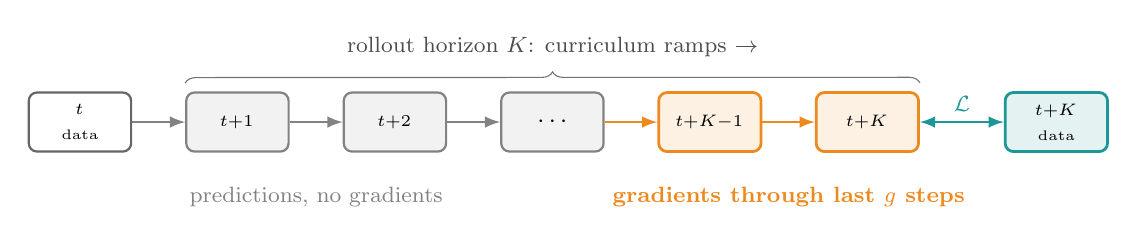
\begin{tikzpicture}[font=\small, >=latex, x=1cm, y=1cm,
    s/.style={rounded corners=3pt,draw=black!60,line width=0.8pt,fill=white,
              align=center,inner sep=4pt,minimum height=0.75cm,minimum width=1.3cm},
    sp/.style={rounded corners=3pt,draw=rollpred,line width=0.8pt,fill=black!5,
               align=center,inner sep=4pt,minimum height=0.75cm,minimum width=1.3cm},
    sg/.style={rounded corners=3pt,draw=rollgrad,line width=1pt,fill=rollgrad!12,
               align=center,inner sep=4pt,minimum height=0.75cm,minimum width=1.3cm},
    tr/.style={rounded corners=3pt,draw=rolltgt,line width=1pt,fill=rolltgt!12,
               align=center,inner sep=4pt,minimum height=0.75cm,minimum width=1.3cm}]

  %% Rollout chain: data -> no-grad predictions -> grad steps -> target
  \node[s]  (x0) at (0,0)     {$\state_t$\\[-1pt]{\tiny data}};
  \node[sp] (x1) at (2.0,0)   {$\shat_{t+1}$};
  \node[sp] (x2) at (4.0,0)   {$\shat_{t+2}$};
  \node[sp] (x3) at (6.0,0)   {$\cdots$};
  \node[sg] (x4) at (8.0,0)   {$\shat_{t+K-1}$};
  \node[sg] (x5) at (10.0,0)  {$\shat_{t+K}$};
  \node[tr] (xt) at (12.4,0)  {$\state_{t+K}$\\[-1pt]{\tiny data}};

  \draw[->,line width=0.9pt,rollpred] (x0) -- (x1);
  \draw[->,line width=0.9pt,rollpred] (x1) -- (x2);
  \draw[->,line width=0.9pt,rollpred] (x2) -- (x3);
  \draw[->,line width=0.9pt,rollgrad] (x3) -- (x4);
  \draw[->,line width=0.9pt,rollgrad] (x4) -- (x5);
  \draw[<->,line width=0.9pt,rolltgt] (x5) -- node[above,font=\footnotesize]{$\mathcal{L}$} (xt);

  %% Curriculum brace above the rollout
  \draw[decorate,decoration={brace,amplitude=4pt,raise=3pt},black!55]
    (x1.north west) -- (x5.north east)
    node[midway,above=9pt,font=\footnotesize,text=black!70]
    {rollout horizon $K$: curriculum ramps $\kzero \to \kmax$};

  %% Group labels below
  \node[text=rollpred,font=\footnotesize] at (3.0,-0.95)
    {predictions, no gradients};
  \node[text=rollgrad,font=\footnotesize\bfseries] at (9.0,-0.95)
    {gradients through last $g$ steps};

\end{tikzpicture}

  \caption{Pushforward rollout training with a horizon curriculum. The surrogate
    is unrolled autoregressively from a data state $\state_t$; the first
    $K-g$ steps are executed without gradients (grey) and only the final
    $g=2$ steps carry gradients (orange). The MSE loss $\mathcal{L}$ is applied
    at the terminal prediction $\shat_{t+K}$ against the data target
    $\state_{t+K}$. A curriculum ramps the rollout horizon $K$ from $\kzero$ to
    $\kmax$ over training, exposing the model to its own prediction errors
    without backpropagating through the full rollout graph.}
  \label{fig:pushforward}
\end{figure}

A naive one-step training objective, where the network always receives a
ground-truth state as input, produces models that degrade rapidly during
autonomous multi-step rollout because the network never learns to handle its
own prediction errors \cite{brandstetter2022}. The pushforward trick addresses
this by training with rollouts of length $K$: the network autoregressively
generates a sequence of $K$ predictions and the loss is applied at the terminal
step. The rollout is
\begin{equation}
  \shat_{t+k+1}
    = \fsur(\shat_{t+k},\,\bth_{t+k},\,\mask),
  \qquad k = 0, \ldots, K-1,
  \label{eq:rollout}
\end{equation}
where $\fsur$ denotes the full surrogate step (Eq.~\ref{eq:step}). To
balance exposure to compounding errors against training stability and memory
cost, only the last $g=2$ steps of the rollout carry gradients; earlier
steps are detached from the computational graph. This \emph{truncated}
backpropagation-through-time strategy limits the gradient path length while
retaining sensitivity to error accumulation at the tail of the sequence.

The rollout horizon is annealed by a \emph{curriculum}: $K$ starts at
$\kzero = 2$ and is incremented by one step every $15$ epochs until it reaches
$\kmax = 7$. Early in training the model sees only short, manageable
sequences; as training progresses the horizon grows, forcing the model to
remain accurate over longer autonomous trajectories. The curriculum schedule
and gradient flow are illustrated in Figure~\ref{fig:pushforward}.

\subsubsection{Optimisation and Learning-Rate Schedule}
\label{sec:optim}

The model is trained with AdamW ($\eta = 10^{-4}$, weight decay $= 10^{-8}$)
for up to $200$ epochs with early stopping at patience $15$. The learning-rate
schedule comprises a linear warm-up phase over the first $5$ epochs
($\eta: 10^{-6} \to 10^{-4}$) followed by cosine annealing to $10^{-6}$
for the remainder of training. The warm-up prevents large gradient updates
from destabilising the randomly initialised network in the first few iterations,
while the cosine decay provides a smooth final refinement phase.

Mixed-precision training uses \texttt{bfloat16} automatic mixed precision
(bf16 AMP), which reduces memory bandwidth pressure and enables larger batch
sizes compared to full precision without the numerical range issues that can
affect fp16 on large activations. The model is compiled with
\texttt{torch.compile(dynamic=False)}, which generates optimised CUDA kernels
for the fixed input shapes of our domain and typically yields a $20$--$40\%$
throughput improvement. Gradient norms are clipped to $1.0$ to prevent
occasional spikes during the later curriculum stages from corrupting the model
weights.

\subsection{Fine-Tuning}
\label{sec:finetuning}

% TODO: describe fine-tuning of a pretrained surrogate (e.g. adapting a base
% model to a specific geometry, inflow regime, or higher-fidelity data with a
% short low-learning-rate continuation of training). Placeholder for now.
\textit{This section is under preparation: it will describe how a pretrained
surrogate is fine-tuned---for example to specialise a base model to a particular
geometry or inflow regime---before it is deployed.}

\subsection{Training Across Geometries}
\label{sec:multigeom}

% TODO: describe geometry-generalising / multi-geometry training (conditioning
% the surrogate on the geometry mask across several urban blocks so a single
% model transfers between sites). Placeholder for now.
\textit{This section is under preparation: it will describe how the surrogate is
trained across multiple building geometries so that a single model generalises
between urban sites rather than being tied to one domain.}

\subsection{Training Data Generation}
\label{sec:data}

Training trajectories are generated by running the \palm{} LES solver
\cite{maronga2020} over the Barcelona domain under a diverse set of inflow
conditions. For each training simulation the inflow angle $\iang$ and velocity
magnitude $\ivel$ are drawn from AR(2) processes (Section~\ref{sec:prior}), with
external means sampled
independently per trajectory: $\mu_\alpha \sim \mathcal{U}(-25^\circ, 25^\circ)$
and $\mu_V \sim \mathcal{U}(5\,\mathrm{m/s},\,10\,\mathrm{m/s})$. The
process noise standard deviations are $\sigma_\alpha = 5^\circ$ and
$\sigma_V = 0.5\,\mathrm{m/s}$, producing realistic time-varying inflow
sequences while covering the plausible range of urban boundary-layer conditions.
Velocity snapshots and corresponding inflow parameter sequences are saved at
fixed output intervals and constitute the supervised training set.
